\section{City Block Generation}

Once roads and streets have been generated, the city block generation starts.
This generation step produces a list of polygons that mark which areas of the terrain are suitable for buildings, parks, and parking lots.
City blocks may vary significantly in size, but a limit is set on how large they can become (see Figure \ref{fig:results_blockgen1}).

% TODO: Replace this figure, it has some inset problems.
\begin{figure}[h!]
  \centering

  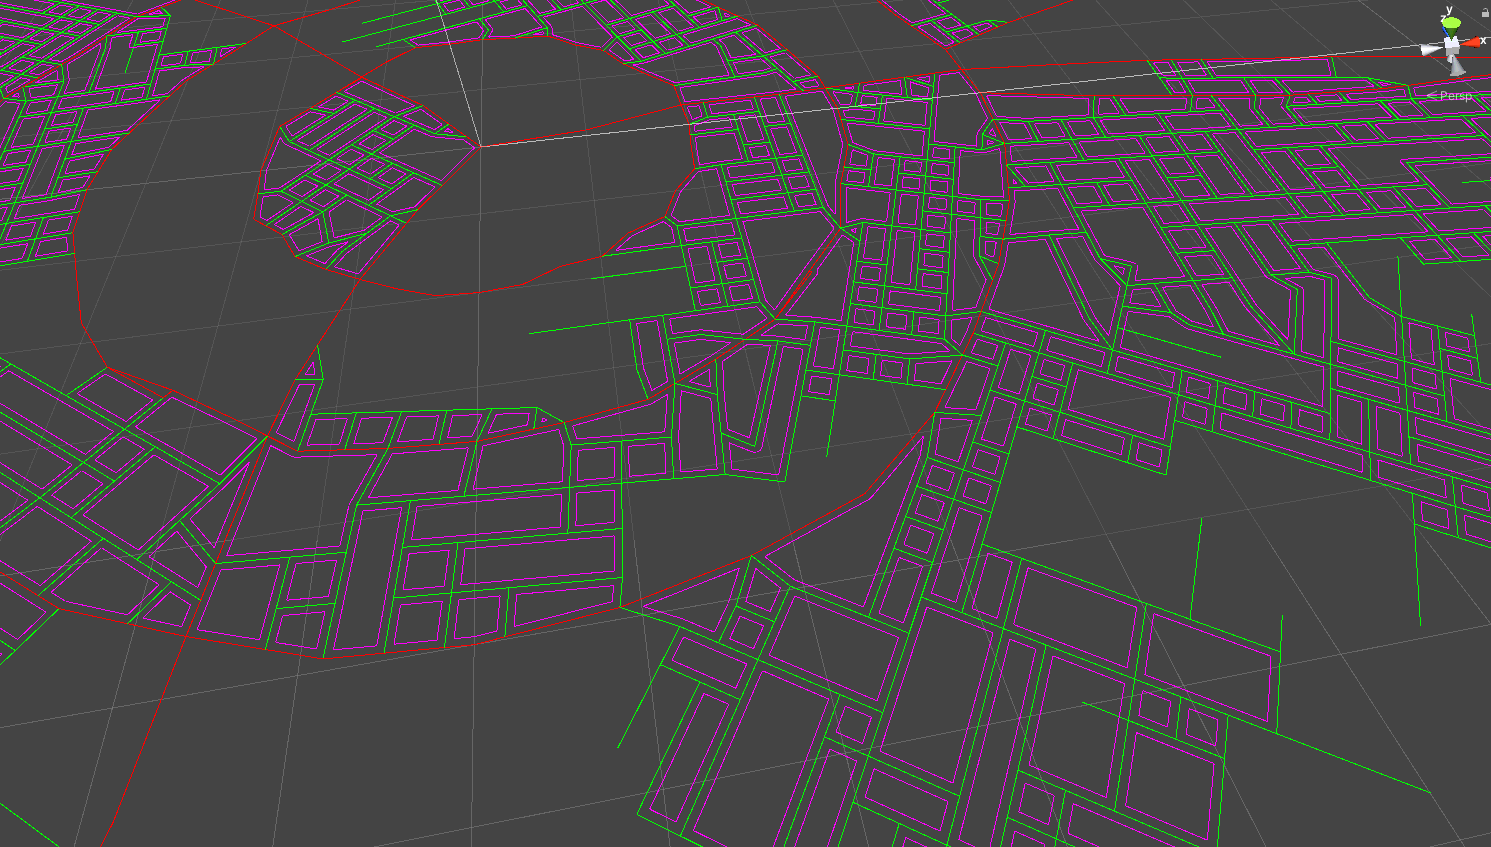
\includegraphics[width=0.8\textwidth]{figure/results_blockgen1.png}
  \caption{Generation of city blocks on a flat road network. Red and green lines represent roads and streets respectively, while pink lines are city blocks. Notice how the largest areas are not treated as blocks.}

  \label{fig:results_blockgen1}
\end{figure}

Each city block is also guaranteed to be connected to the road network, such that roads, streets, or both surround it.
Consequently, each block has to be slightly inset in order to make room for the road meshes.
This necessity becomes more apparent when all meshes are rendered (see Figure \ref{fig:results_blockgen2}).

\begin{figure}[h!]
  \centering

  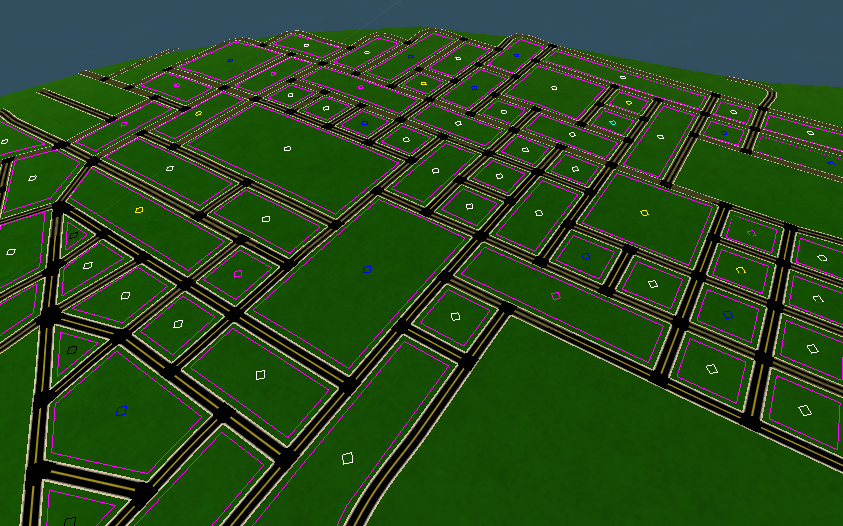
\includegraphics[width=0.9\textwidth]{figure/results_blockgen2.png}
  \caption{Blocks generated on a 3D terrain. Notice how each block is connected to the road network. Green and pink lines are only shown during development.}

  \label{fig:results_blockgen2}
\end{figure}

Each city block is assigned a label that helps the subsequent plot generation step determine what to generate inside each city block.
In Figure \ref{fig:results_blockgen2} these labels are visualized as green triangles, meaning they have not been processed yet.
The green triangles are also used to mark blocks that became too small after being inset, effectively excluding them from further processing.
An example of this behavior is shown in Figure \ref{fig:results_blockgen3}.

\begin{figure}[h!]
  \centering
  \begin{subfigure}[b]{0.47\textwidth}
    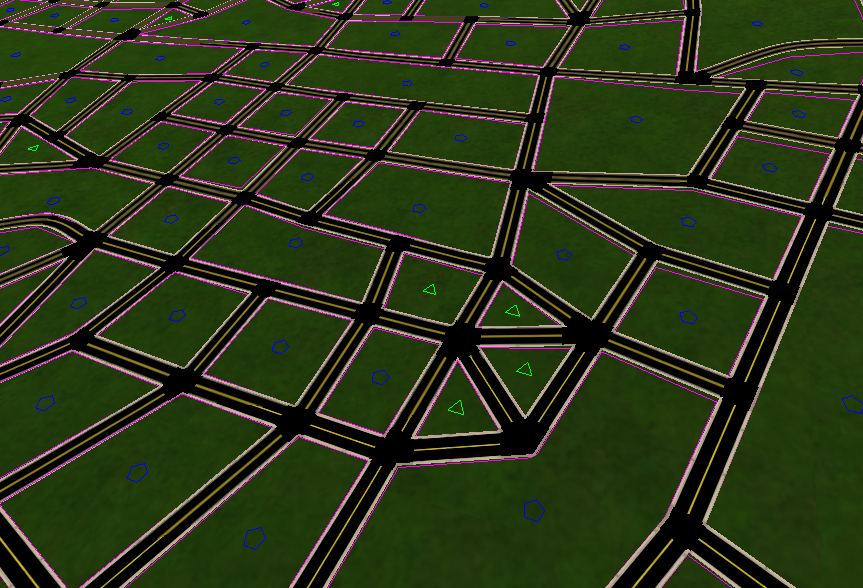
\includegraphics[width=\textwidth]{figure/results_blockgen3.png}
  \end{subfigure}
  \quad
  \begin{subfigure}[b]{0.45\textwidth}
    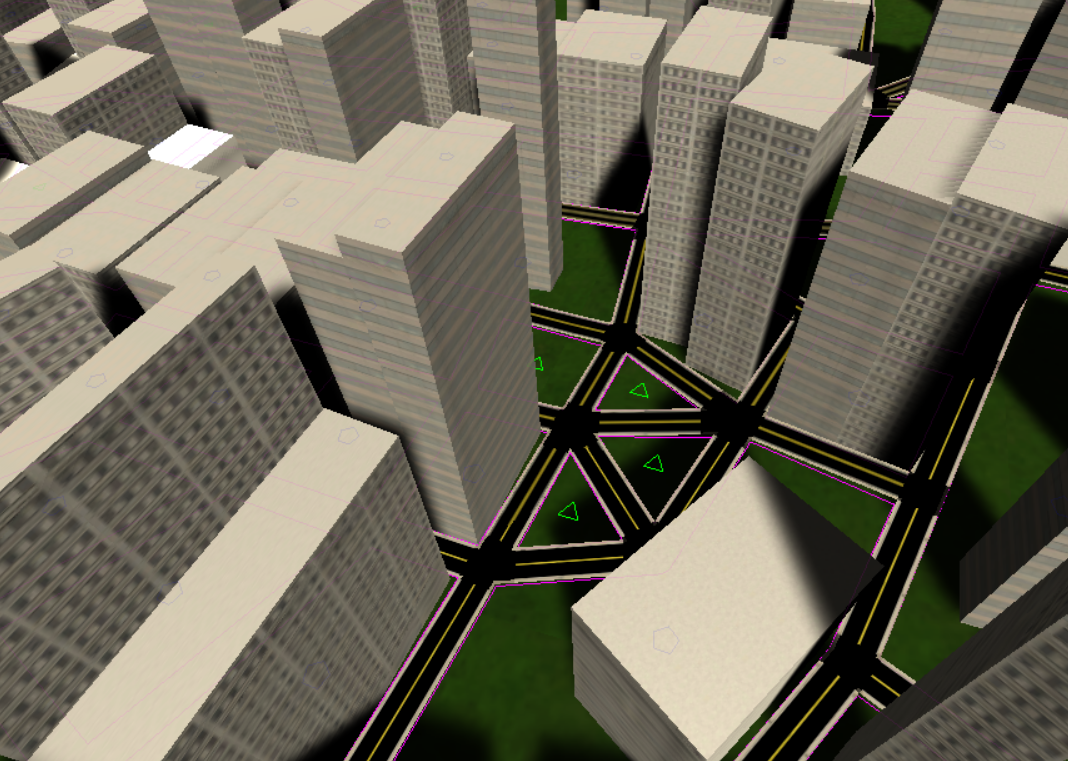
\includegraphics[width=\textwidth]{figure/results_blockgen4.png}
  \end{subfigure}

  \caption{City blocks with different labels (green/blue) shown without (left) and with (right) buildings rendered. Blocks with green labels are too small, and blocks with blue labels have the \textit{skyscrapers} label.}
  \label{fig:results_blockgen3}
\end{figure}

The implemented labels are \textit{industrial}, \textit{surburbs}, \textit{downtown}, \textit{skyscrapers}, \textit{apartments} and \textit{parks}.
Each label weights what type of content should be generated so that all plots within the same block share a certain theme.
Finally, once the blocks are generated, they are passed on to the plot generation.